\documentclass{article}
\title{Bagged indicator function}
\usepackage{amsmath}
\usepackage{bbm}
\usepackage{graphicx}
\begin{document}
\maketitle
\begin{align*}
\hat{\theta}_n(x) &= \mathbbm{1}_{\{\bar{Y_n} \leq x\}}\\
\frac{\sqrt{n}(\bar{Y_n}- \mu)}{\sigma} &\overset{D}{\rightarrow} N(0,1)\\
\intertext{Take x in the $n^{-1/2}$ neighborhood of $\mu$}
x &= x_n(c) = \mu + c\sigma n^{-1/2}\\
\hat{\theta}_n(x_n(c)) &=\mathbbm{1}_{\{\bar{Y_n}\leq\mu+c\sigma n^{-1/2}\}}\\
&=\mathbbm{1}_{\{\frac{\sqrt{n}(\bar{Y_n} - \mu)}{\sigma}\leq c\}}\\
&\approx \mathbbm{1}_{\{Z\leq c\}}\\
\intertext{This gives us}
E(\hat{\theta}_n(x_n(c))) &\rightarrow P[Z\leq c] = \Phi(c)\,\, \text{and}\,\, Var(\hat{\theta_n}(x_n(c))) &\rightarrow \Phi(c)(1- \Phi(c))\\
\intertext{Now consider the bagged estimator}
\hat{\theta}_{B;n}(X_n(c)) &= E^{\star}[\mathbbm{1}_{\{\bar{Y_n^{\star}}\leq x_n(c)\}}]\\
&= E^{\star}[\mathbbm{1}_{\{\frac{\sqrt{n}(\bar{Y_n}^{\star} -\bar{Y_n})}{\sigma}\leq \frac{\sqrt{n}(x_n(c) - \bar{Y_n})}{\sigma}\}}]\\
&=\Phi\left(\frac{\sqrt{n}(x_n(c) - \bar{Y_n})}{\sigma}\right) + o_p(1)\\
&\overset{D}{\approx}\Phi(c-Z)\\
\hat{\theta}_{n;B}(x_n(0)) &\rightarrow \Phi(-Z) = U[0,1]\\
E(\hat{\theta}_{n;B}(x(0)) = 1/2 \text{So unbiased!}\\
Var(\hat{\theta}_{n;B}(x(0)) = 1/12\\ 
\intertext{Reduction in variance by a factor of 3!}
\end{align*}

\newpage
\begin{figure}
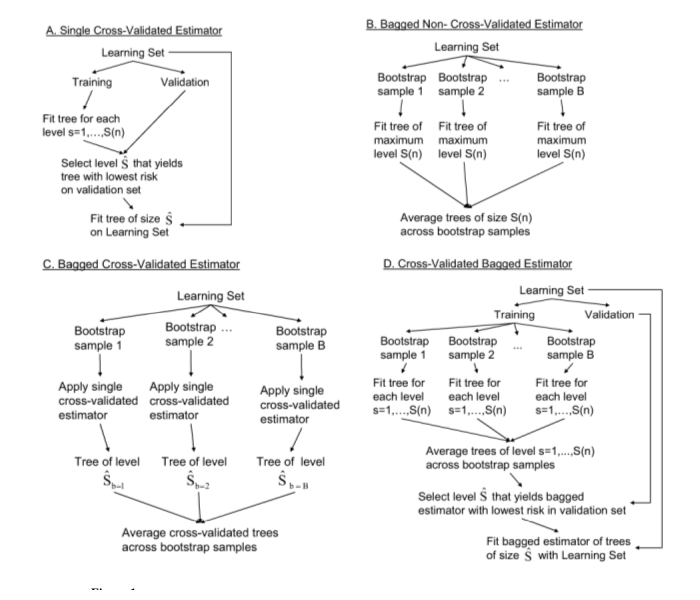
\includegraphics[width=0.9\textwidth]{PetersenFig1.png}
\caption{Flowcharts for bootstrap and cross-validation, from [2].}
\end{figure}

References:

[1] Buhlmann, P. and Yu, B. (2002). Analyzing bagging. \emph{Ann.
  Statist.} \textbf{30} 927-961.

[2] Petersen, M. L., Molinaro, A. M., Sinisi, S. E., van derLaan, M.
J. Cross-Validated Bagged Learning. \emph{J Multivar Anal.} (2008). 25(2): 260-266


\end{document}
